\chapter{Extrahierung}

Der nächste Schritt auf dem Weg zum finden eines gültigen \QRCodes besteht darin, alle Möglichen Dreier-Kombinationen von \fps zu prüfen und festzustellen, ob diese zur Extrahierung eines gültigen \QRCodes führen. Für jede Kombination wird versucht, die vier Eckpunkte des \QRCodes zu berechnen, um aus diesem eine Matrix für eine perspektivische Transformation in eine 2D-Ebene zu berechnen. Dies führt zu $\binom{k}{3}$ möglichen Kombinationen von \fps, wobei $k$ die Anzahl aller gefundenen \fps ist.

\section{Pattern Positionierung}
Hat man drei \fps ausgewählt, muss für die korrekte Extrahierung festgestellt werden, welche Position im \QRCode jedes \fp einnimmt.

Zuerst werden dazu die \fps durch Verwendung der Gaußschen Trapezformel im Uhrzeigersinn angeordnet.
\begin{theorem}[Gaußsche Trapezformel]
Berechnet den Flächeninhalt eines einfachen Polygons.
\begin{align}
A=\frac{1}{2} \sum_{0}^{n-1} (y_i + y_{i+1\ mod\ n})(x_i - x_{i+1\ mod\ n})
\end{align}
\end{theorem}
Dabei ist $n$ die Anzahl der Punkte in einem Polygon und $x_i$ und $y_i$ die Punktkoordinaten des $i$-ten Punkts. Abhängig vom Drehsinn der Punkte im Bezug auf das Koordinatensystem ist der Flächeninhalt entweder positiv oder negativ. In einem kartesischen Koordinatensystem entspricht ein positiver Flächeninhalt einem Drehsinn im Uhrzeigersinn und ein negativer gegen den Uhrzeigersinn.

Angewendet wird die Formel auf das Polygon, welches aus dem jeweils ersten Punkt der Kontur jedes \fps besteht. Ist der Flächeninhalt negativ wird die Reihenfolge geändert, indem das erste und zweite \fp miteinander vertauscht werden.
\subsubsection{Ähnlichkeitsmaß für Geraden}
Sind die \fps in korrekter Reihenfolge, wird als nächstes das \olfp bestimmt. Zurzeit sind durch die drei \fps insgesamt 12 approximierte Geraden bekannt. Betrachtet man den Aufbau eines \QRCodes, ist ersichtlich das jeweils 4 Geradenpaare die selbe Kante beschreiben. Es gibt insgesamt also nur 8 unterschiedliche Kanten und nur das \olfp teilt sich jede Kante mit einem anderen \fp. Die anderen beiden \fps teilen sich je nur 2 Kanten mit dem \olfp. Stellt man also fest welche der 12 Geraden die gleichen Kanten im \QRCode approximieren, ergibt sich welches \fp das \olfp ist.

Für das effiziente Zuordnen von Geraden wird ausgenutzt, dass die Stützvektoren der Kantengeraden stets im Mittelpunkt der Segmente liegen durch welche sie approximiert wurden. Die Ähnlichkeit von zwei Geraden wird dann definiert über die Summe der Entfernung des Stützvektors der ersten Gerade zur zweiten Gerade und umgekehrt.

\inputCPP[label={lst:similarity}][][Ähnlichkeitsmaß für zwei Geraden]{code/similarity.cpp}

\begin{wrapfigure}{R}{0.4\textwidth}
  \vspace{-20pt}
  \begin{center}
    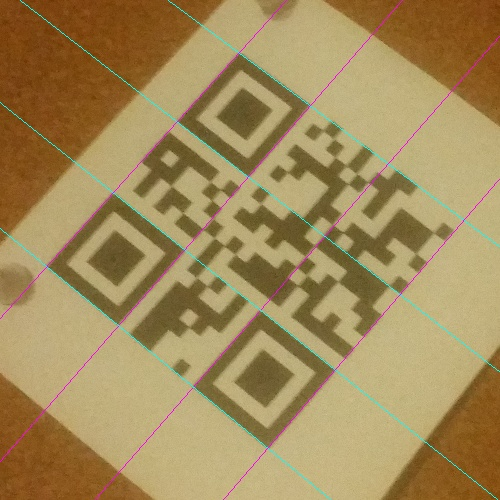
\includegraphics[scale=0.25]{images/qrcode-adler-wand_6___SPLIT___0_.jpg}
  \end{center}
  \vspace{-10pt}
  \caption{Zuordnung der Geraden zu horizontalen oder vertikalen Kanten.}
  \vspace{-10pt}
\end{wrapfigure}

Ein kleinerer Wert bedeutet bei dieser Definition das sich zwei Geraden besonders ähnlich sind. In Abbildung \ref{fig:lines} ist dabei gut zu erkennen, dass wenn es sich um einen \QRCode handelt, welcher mit ausreichend guter Qualität für eine korrekte Kantenapproximation abgebildet ist, sich dieses Maß ausreichend gut eignet um festzustellen, welche Geraden die selbe Kante approximieren. Für das \olfp gilt dann, dass es das \fp mit den vier kleinsten Ähnlichkeitsmaßen ist.

Da zuvor die \fps im Uhrzeigersinn angeordnet wurden, können wir durch Rotation im Uhrzeigersinn nicht nur das \olfp an die erste Stelle des Pattern Arrays bringen, sondern wissen auch direkt das sich an der zweiten Stelle das \orfp und an der dritten Stelle das \ulfp befindet. Mit Ausnahme für Spiegel verkehrte \QRCodes kann zuverlässig die korrekte Position aller \fps im \QRCode bestimmt werden.

\begin{figure}[h]
\center
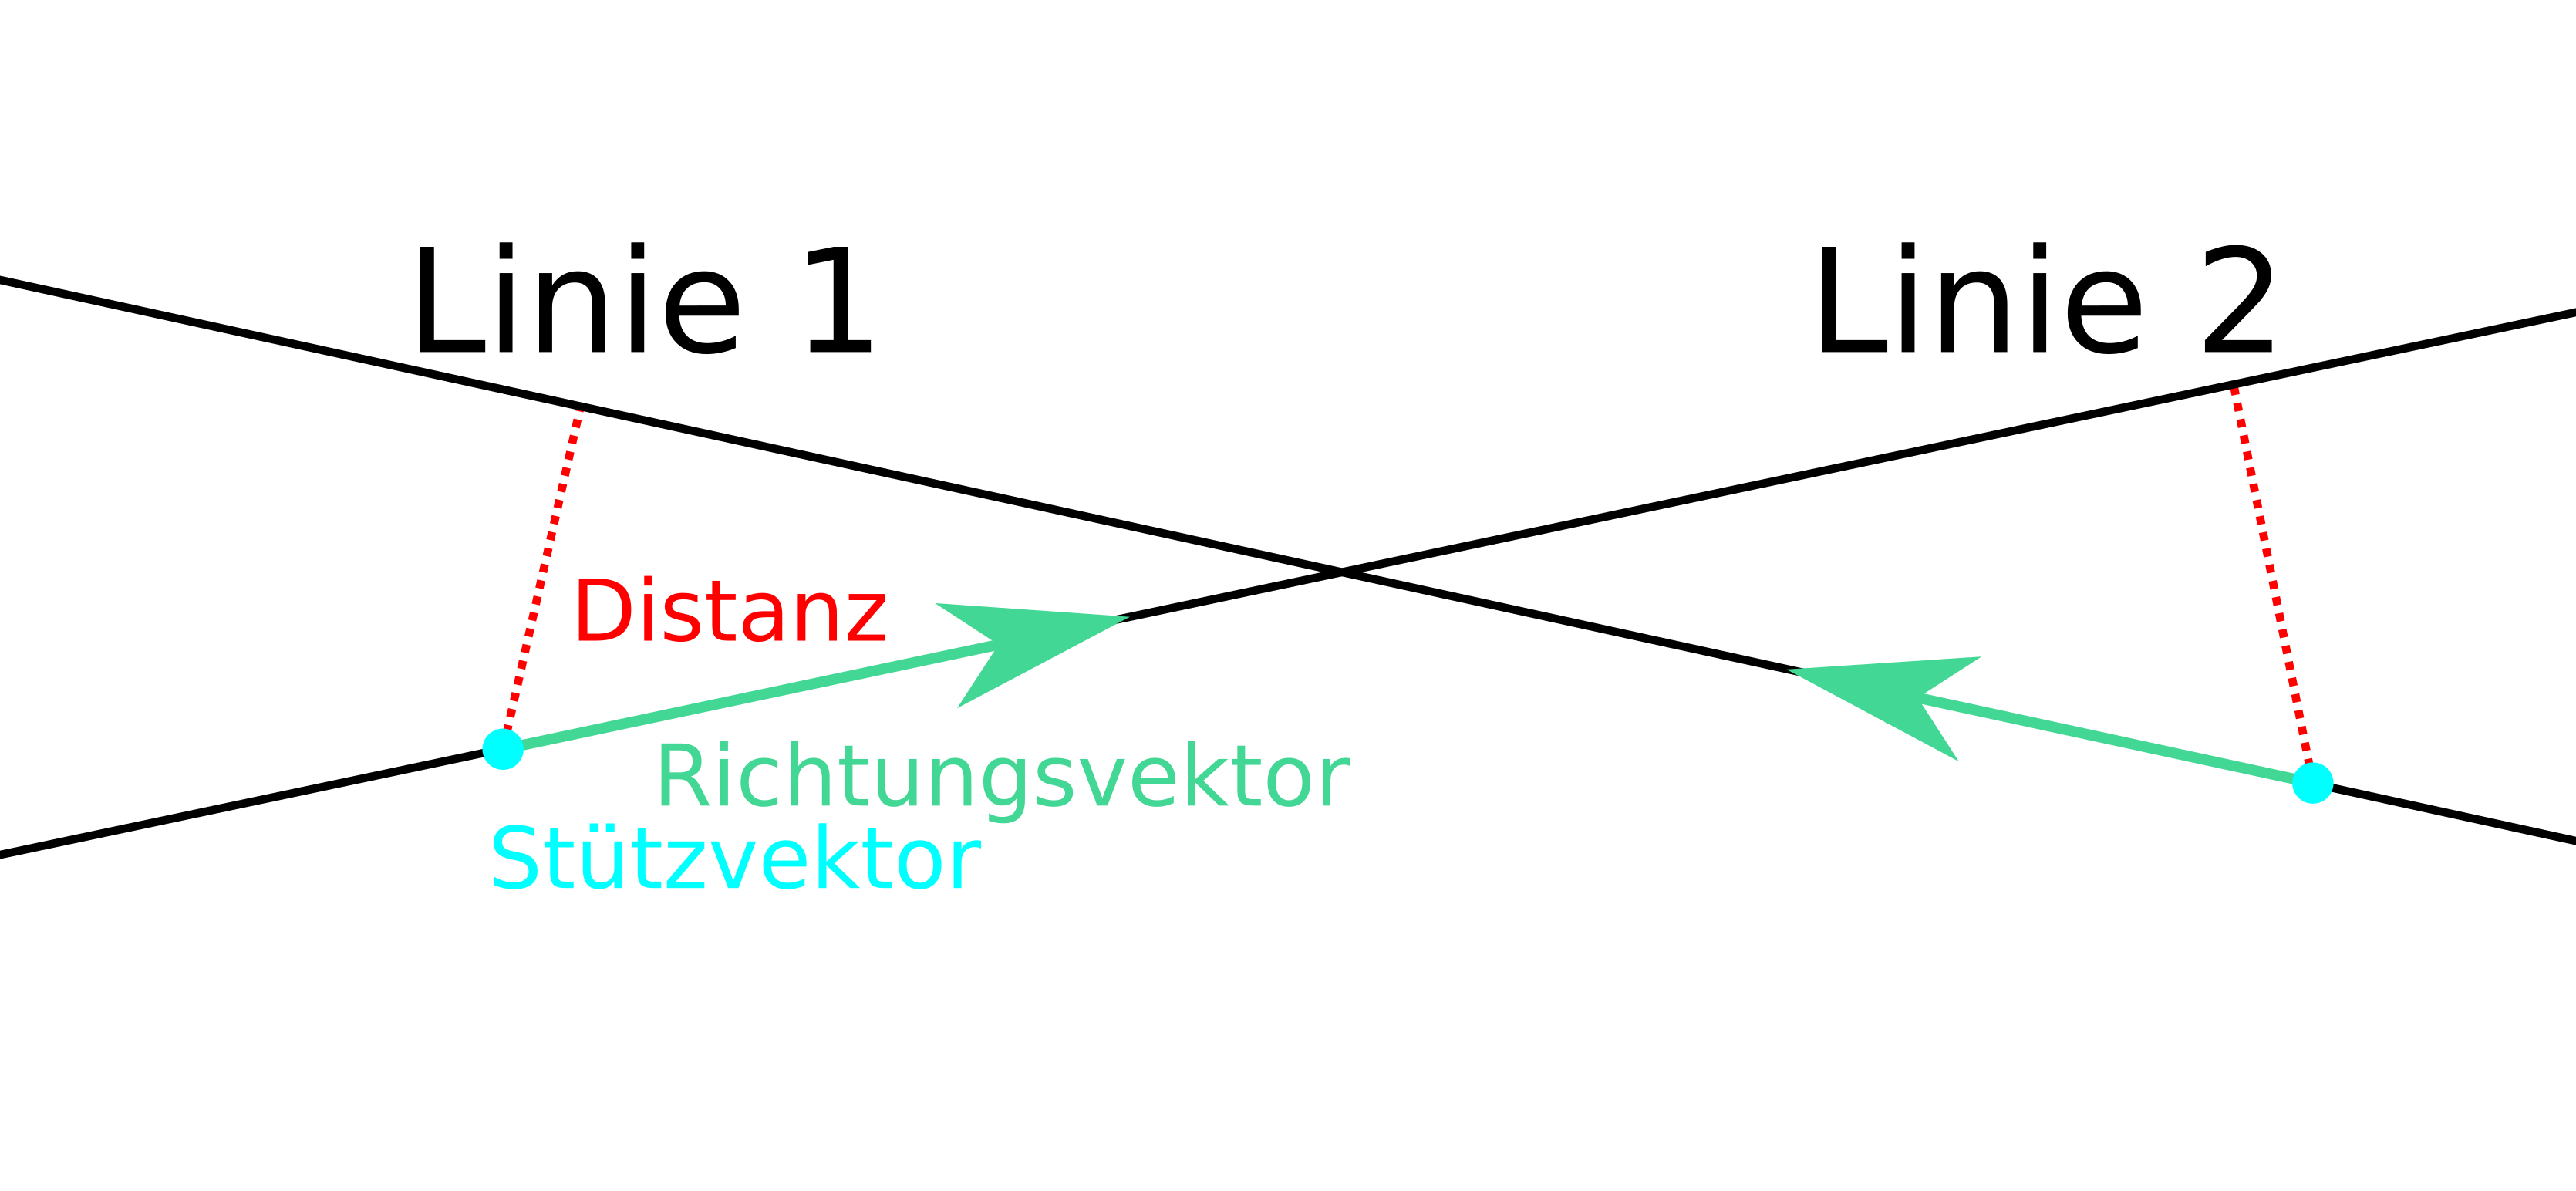
\includegraphics[scale=1]{images/similarity_measure.png}
\caption{Links: Ähnlichkeitsmaß von zwei Geraden.}
\end{figure}

\section{Kanten Zuordnung}
Um die Eckpunkte des \QRCodes durch Schnittpunktbildung der äußeren Kanten zu berechnen, muss als nächstes festgestellt werden, welche Geraden die Außenkanten des \QRCodes beschreiben.

\subsubsection{Vertikale und Horizontale Geraden}
Da bereits berechnet wurde, welche der Geraden die selbe Kante approximieren, kann diese Information benutzt werden um eine qualitativ bessere Approximation für alle Kanten des \olfp zu berechnen. Dazu werden die zugrunde liegenden Segmente von den gepaarten Geraden genommen und auf der Vereinigung dieser Segmente wird erneut der Approximationsprozess ausgeführt. Indem dabei festgestellt wird ob mit einer Geraden aus dem \orfp oder dem \ulfp vereinigt wird, ergibt sich ob die neue Gerade im \QRCode Koordinatensystem eine horizontale oder vertikale Kante beschreibt. Die nicht verwendeten Kanten am Ende des Prozesses sind danach ebenfalls trivial zuzuordnen. Falls an dieser Stelle nicht genau je zwei Geradenpaare von \olfp und \orfp, sowie zwei Geradenpaare von \olfp und \orfp vereinigt wurden, ist die Kombination von \fps kein \QRCode und es kann abgebrochen werden.

War die Vereinigung erfolgreich gibt es genau vier horizontal und vier vertikal zugeordnete Geraden.

\subsubsection{Sortieren der Geraden}
Danach werden die horizontalen Geraden entlang einer beliebigen vertikalen Gerade sortiert, welche von nun an als Sortier-Achse bezeichnet wird. 

Wie in Abbildung \ref{fig:sort} gezeigt, werden dazu alle Schnittpunkte zwischen der Sortier-Achse und den horizontalen Geraden berechnet. Dann wird eine Koordinatensystem Transformation ausgeführt, sodass die Sortier-Achse zur neuen X-Achse des Koordinatensystems wird. Somit können die horizontalen Geraden nach der Größe der X-Werte der Schnittpunkte mit der Sortier-Achse sortiert werden. Zuletzt wird festgestellt ob das erste Element der so sortierten Liste von horizontalen Geraden mit einer Gerade des \olfp übereinstimmt. Falls nicht wird die Liste umgedreht.

Für die vertikalen Geraden kann dies analog durchgeführt werden. Diese Methode wurde gewählt, um sicherzustellen das unabhängig von perspektivischen Verzerrungen die Sortierreihenfolge stabil bleibt.

\begin{figure}[h]
\centering
\begin{subfigure}[t]{0.48\textwidth}
\centering
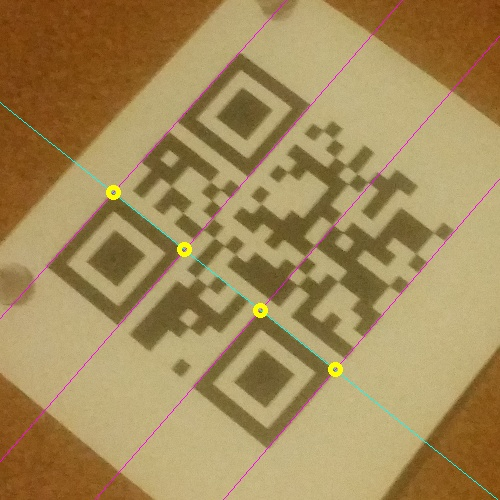
\includegraphics[scale=0.25]{images/qrcode-adler-wand_7___SORT___0_.jpg}
\caption{Schnittpunkte entlang der Sortier-Achse}\label{fig:sort}
\end{subfigure}%
\begin{subfigure}[t]{0.48\textwidth}
\centering
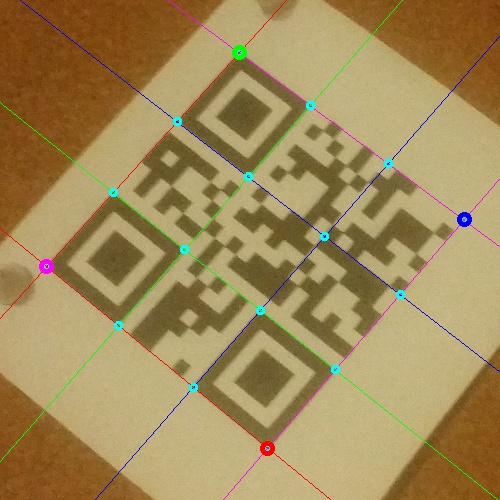
\includegraphics[scale=0.25]{images/qrcode-adler-wand_9___INTERSECTIONS___0_.jpg}
\caption{Schnittpunkte aller horizontalen und vertikalen Geraden}
\end{subfigure}
\caption{Sortieren aller Geraden entlang einer Achse und Berechnung der Eckpunkte.}
\end{figure}

Das Ergebnis sind zwei Listen von Geraden die im \QRCode Koordinatensystem von oben links nach unten rechts sortiert sind. Dementsprechend können nun trivial die Schnittpunkte der ersten und letzten Geraden berechnet werden, wodurch die Eckpunkte des \QRCodes bestimmt werden. Mit diesen vier Punkten und der \OpenCV Funktion  \texttt{getPerspectiveTransform} sowie \texttt{warpPerspective} wird dann eine perspektivische Transformationsmatrix errechnet und der \QRCode extrahiert.